\section{See-Saw method of finding weighted average}

As the name suggests, this is a method that resembles a see-saw. A see-saw is a horizontal bar where at the end, weights are put on. To keep the see-saw balanced, either the weights must be equal or the "torque" must be equal

\begin{figure*}[h!]
    \centering
    % 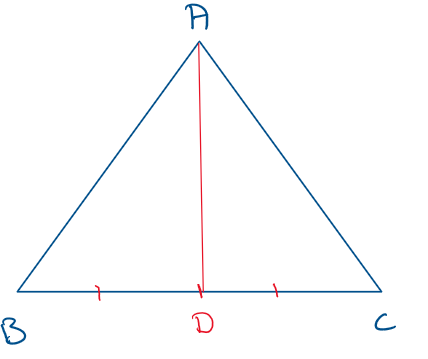
\includegraphics[width=0.25\linewidth]{Quant//Geometry//Images//Triangles/triangle_median_intro.png}
    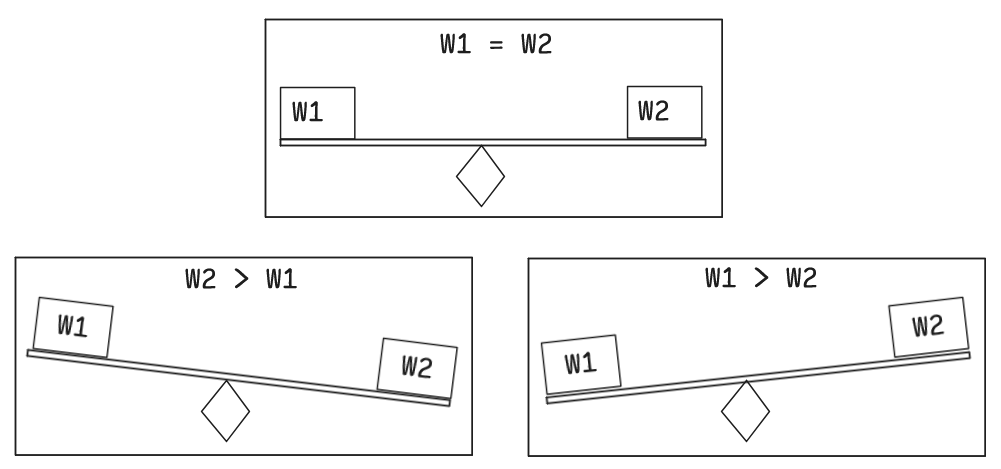
\includegraphics[width=0.50\linewidth]{Quant//Arithmetic//IMAGES//alligation_see_saw_basic.png}
\end{figure*}

The torque is defined as "Weight * distance from center". The weight $w$ and the distance $d$ from center are inversely proportional to each other


\begin{itemize}
    \item If $W_1 > W_2$ then $W_1 * d_1 > W_2 * d_2$.
    \item However, to keep the see-saw in equilibrium, the torque must be same
    \item To keep the torque same, $d_1 < d_2 \implies W_1 * d_1 = W_2 * d_2$
    \item We can say that $W \propto \dfrac{1}{d} \implies W_1 * d_1 = W_2 * d_2 \implies \dfrac{W_1}{W_2} = \dfrac{d_2}{d_1}$
\end{itemize}

\begin{figure*}[h!]
    \centering
    % 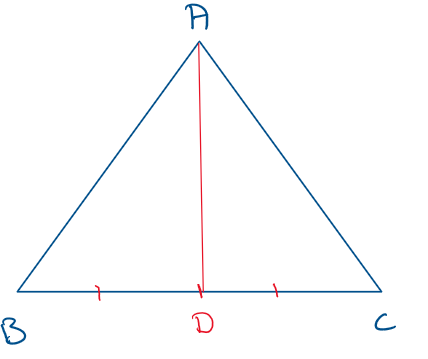
\includegraphics[width=0.25\linewidth]{Quant//Geometry//Images//Triangles/triangle_median_intro.png}
    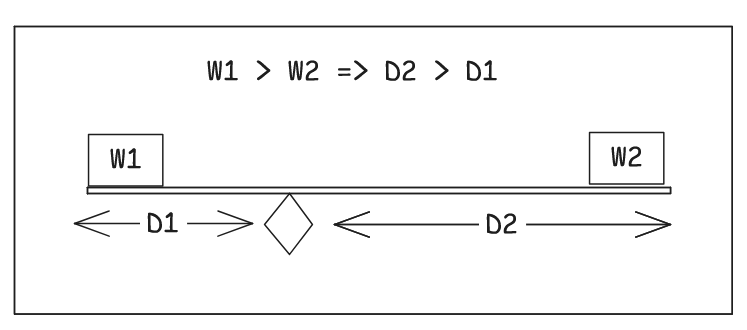
\includegraphics[width=0.50\linewidth]{Quant//Arithmetic//IMAGES//alligation_see_saw_distance.png}
\end{figure*}

\newpage

Using the ratio of weights, we can determine ratio of distances. To solve our questions, we will put another attribute on weight called "Price". Sum of distances will be equal to the difference of the prices $\implies d_1 + d_2 = p_2 - p_1$

\begin{figure*}[h!]
    \centering
    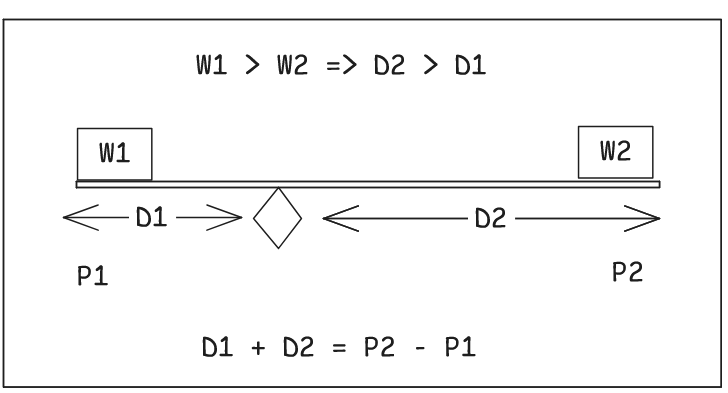
\includegraphics[width=0.50\linewidth]{Quant//Arithmetic//IMAGES//alligation_see_saw_distance_price.png}
\end{figure*}

\SampleQuestion{68Kg of apples are sold at Rs 63/Kg and 85Kg of apples are sold at Rs 81/Kg. Find average price}

\begin{multicols}{2}
    
    \textbf{Standard Method}
    
    We can find weighted average as follows
    \begin{align*}
        &= \dfrac{(68 * 63) + (85 * 81)}{68 + 85} \\
        &= \dfrac{17 * (4 * 63 + 5 * 81)}{17 * (4 + 5)} \\
        &= \dfrac{252 + 405}{9} \\
        &= 73
    \end{align*}
    
    \columnbreak
    
    \textbf{See-Saw Method}
    
    \begin{itemize}
        \item Weights = 68 Kg, 85 Kg
        \item Price = Rs 63/Kg, Rs 81/Kg
        \item $\dfrac{d_2}{d_1} = \dfrac{W_1}{W_2} \implies \dfrac{68}{85} \implies \dfrac{4}{5}$
        \item Therefore, $d_1 = 5x, d_2 = 4x$
    \end{itemize}

    \begin{itemize}
        \item Now, $d_1 + d_2 = P_2 - P_1 \implies 9x = 81 - 63 \implies x = \dfrac{18}{2} = 2$
        \item Average = $p_1 + d_1 \implies 63 + (5 * 2) = 73$
    \end{itemize}
    
\end{multicols}
    
\begin{figure*}[h!]
    \centering
    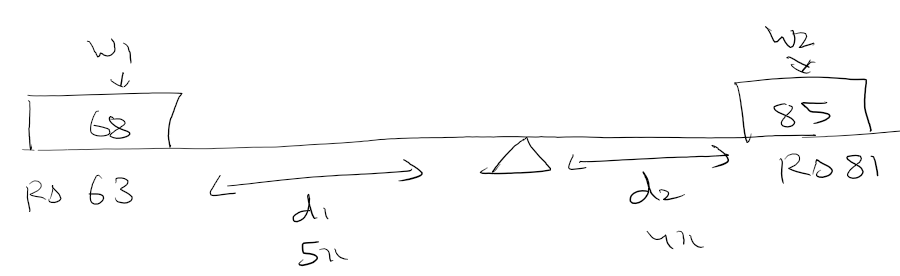
\includegraphics[width=0.5\linewidth]{Quant//Arithmetic//IMAGES//alligation_q1_1.png}
\end{figure*}



\SampleQuestion{27 boys have 70 marks as average and 18 girls have 80 marks average. Find average of class}

\begin{figure*}[h!]
    \centering
    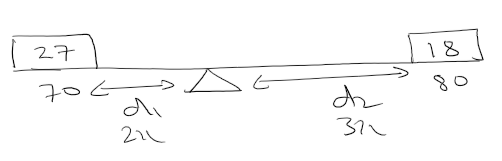
\includegraphics[width=0.5\linewidth]{Quant//Arithmetic//IMAGES//alligation_q2_1.png}
\end{figure*}


\begin{multicols}{2}

    \begin{itemize}
        \item Weight = quantities, Price = marks 
        \item $W_1 = 27, P_1 = 70$
        \item $W_2 = 18, P_2 = 80$
    \end{itemize}
    
    \columnbreak

    \begin{itemize}
        \item $\dfrac{d_2}{d_1} = \dfrac{W_1}{W_2} \implies \dfrac{27}{18} \implies \dfrac{3}{2}$
        \item $d_1 = 2x, d_2 = 3x$
        \item $d_1 + d_2 = P_2 - P_1 \implies 5x = 10 \implies x = 2$
        \item Average = $P_1 + d_1 \implies 70 + (2 * 2) = 74$
    \end{itemize}

\end{multicols}

